\subsection{Transient analysis of bimaterial plate with a notch}

\paragraph{}
In this last example, we study the transient response of a bimaterial plate with a notch terminating at the material interface.
The crack is assumed to be in material 1 and terminating at the interface between the two materials (see Fig.~\ref{iso_fig:bimaterial_plate_geo_bc}).
The length of the crack is assumed to be b/2 and the width of the notch angle is $\theta = 20^\circ$ .
The inputs and the results are non-dimensional.
The plate consists of two materials with different Young's modulus and the same mass density and Poisson's ratio $\nu = 1/3$.
A state of plane stress condition is assumed and the plate is fixed at the bottom.
    \begin{figure}[h!]
        \begin{subfigure}[b]{0.5\linewidth}
            \centering
            \scalebox{0.5}{
                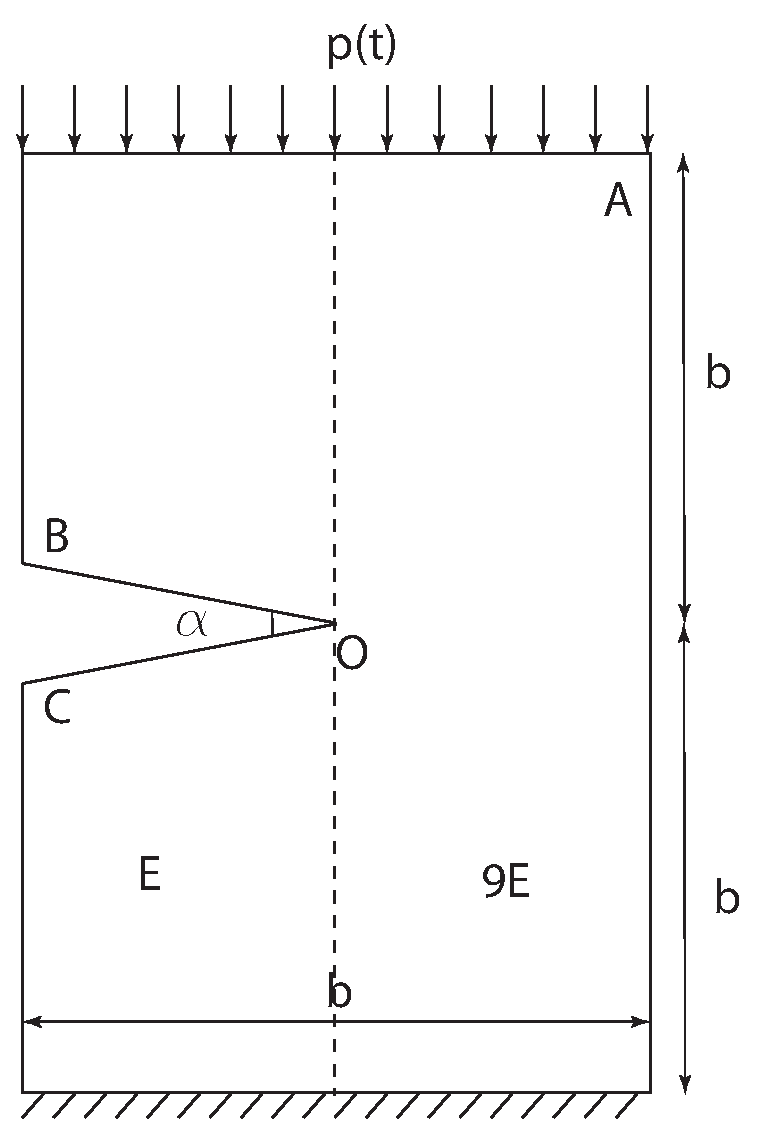
\includegraphics{isogeometric_sbfem/images/bimaterial_plate_geo_bc.eps}
            }
        \end{subfigure}
        \begin{subfigure}[b]{0.5\linewidth}
            \centering
            \scalebox{0.5}{
                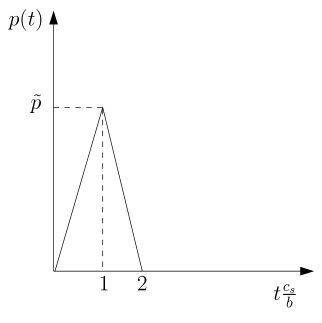
\includegraphics{isogeometric_sbfem/images/bimaterial_plate_load_history.png}
            }
        \end{subfigure}
        \caption{Bimaterial plate with a notch: geometry, boundary conditions and force history}
        \label{iso_fig:bimaterial_plate_geo_bc}
    \end{figure}

\paragraph{}
The main advantage of the proposed method when applied to this example is that, no special treatment is required to represent the weak material discontinuity or the strong discontinuity due to the notch.
The scaling center is placed at the point $O$, where the notch intersects the material interface.
The SBFEM does not require the faces of the notch to be discretized and only the boundary of the domain is discretized.
For this study, the vertical boundaries are discretized using four quartic NURBS functions and the horizontal boundaries are discretized using two quartic
NURBS functions.
Fig.~\ref{iso_fig:bimaterial_plate_natural_frequencies} shows the non-dimensional natural frequencies computed using the proposed method for different orders of continued fractions.
The reference solution is computed by using the commercial software ANSYS$^\circledR$ 14.0.
It is seen that the results from the present approach are in good agreement with the results from the FE software and for the transient analysis, the order of continued fractions is chosen as $M_{cf} = 6$.
    \begin{figure}[h!]
        \centering
        \scalebox{0.4}{
            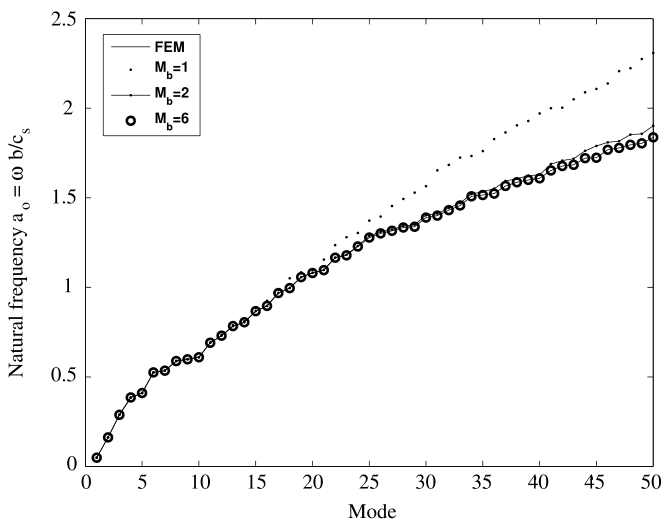
\includegraphics{isogeometric_sbfem/images/bimaterial_plate_natural_frequencies.png}
        }
        \caption{Non-dimensional natural frequencies of a bimaterial plate with a notch}
        \label{iso_fig:bimaterial_plate_natural_frequencies}
    \end{figure}

\paragraph{}
The transient response of the bimaterial plate with a notch is evaluated considering a uniformly distributed load acting at the top horizontal boundary (see Fig.~\ref{iso_fig:bimaterial_plate_geo_bc}).
A triangular impulse load with an amplitude $\widetilde{p}$ with a duration of $2 \times \frac{b}{c_s}$ and peak value $\widetilde{p}$ at time $\widetilde{t}=1\frac{c_s}{b}$ is applied.
The time integration is carried out by employing Newmark's method with $\gamma = 1/2$ and $\beta = 1/4$.
The time step is chosen as $\Delta t = 0.05\frac{b}{c_s}$ and a total of 400 time steps are considered.
The vertical displacement responses at points $A$, $B$ and $C$ are plotted in Fig.~\ref{iso_fig:bimaterial_plate_uy} as functions of the dimensionless time $\widetilde{t} = c_s\frac{t}{b}$
The corresponding results of a finite element analysis are also shown for comparison and an excellent agreement is observed.
The main advantage of the proposed method is that internal discontinuities or material discontinuity does not require special treatment as in other approaches such as the XFEM or the conventional IGA.
Moreover, creating a scaled boundary mesh with NURBS or B-spline functions is straightforward as only the boundary information is required when compared to generating finite element mesh around the notch.
    \begin{figure}[htb]
        \begin{subfigure}[b]{1\linewidth}
            \centering
            \scalebox{0.5}{
                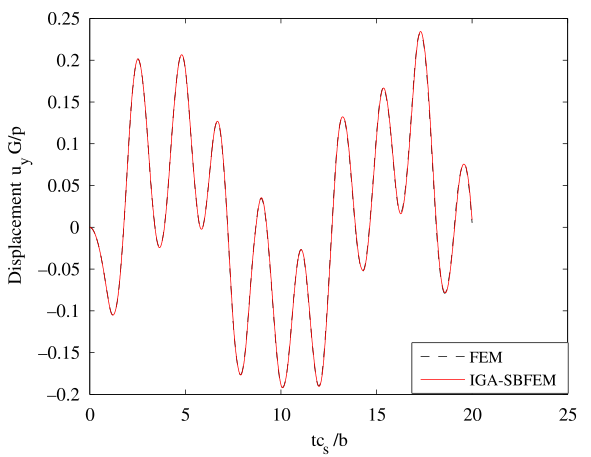
\includegraphics{isogeometric_sbfem/images/bimaterial_plate_uva.png}
            }
            \caption{Point A}
        \end{subfigure}
    
        \begin{subfigure}[b]{1\linewidth}
            \centering
            \scalebox{0.5}{
                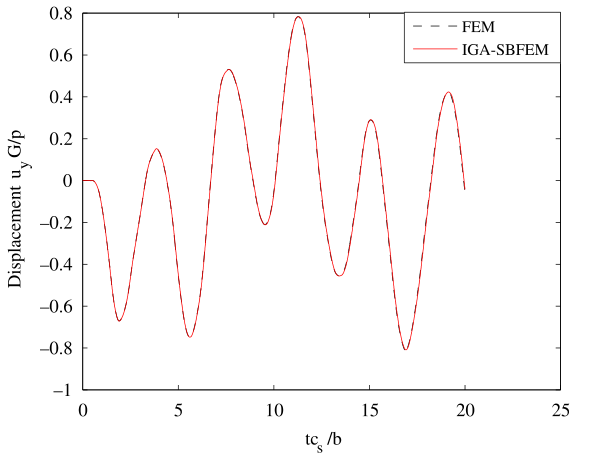
\includegraphics{isogeometric_sbfem/images/bimaterial_plate_uvb.png}
            }
            \caption{Point B}
        \end{subfigure}
    \end{figure}
    \begin{figure}[htb]\ContinuedFloat
        \begin{subfigure}[b]{1\linewidth}
            \centering
            \scalebox{0.5}{
                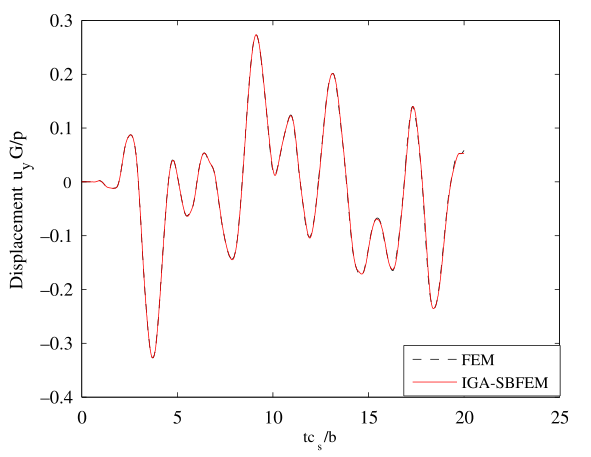
\includegraphics{isogeometric_sbfem/images/bimaterial_plate_uvc.png}
            }
            \caption{Point C}
        \end{subfigure}
    \caption[Vertical displacements of bimaterial plate with a notch]{Vertical displacements of bimaterial plate with a notch at (a) point A; (b) point B; (c): point C}
    \label{iso_fig:bimaterial_plate_uy}
    \end{figure}

